\documentclass[aps,onecolumn,twoside,secnumarabic,balancelastpage,amsmath,amssymb,nofootinbib,hyperref=pdftex]{revtex4}


\usepackage{color}         % produces boxes or entire pages with colored backgrounds
\usepackage{graphics}      % standard graphics specifications
\usepackage[pdftex]{graphicx}      % alternative graphics specifications
\usepackage{longtable}     % helps with long table options
\usepackage[english]{babel}
\setlength{\parskip}{1em}
\usepackage{amsmath}
\usepackage{epsf}          % old package handles encapsulated post script issues
\usepackage{bm}            % special 'bold-math' package
\usepackage{verbatim}			% for comment environment
\usepackage[colorlinks=true]{hyperref}  % this package should be added after all others % use as follows: \url{http://web.mit.edu/8.13}                                    
                                  

\begin{document}
\title{}
\author         {Noah Steinberg}
\email          {nastein@umich.edu}
\date{\today}
\affiliation{University of Michigan - Physics}

\maketitle

\section{Matching SUSY Dimension 5 operators to SMEFT }
When the Heavy colored triplet Higgs is integrated out at the GUT scale, dimension 5 SUSY baryon number violating operators are produced. They are as below,

\begin{equation}
\mathcal{L}^{eff}_{5} = C^{ijkl}_{5L}\mathcal{O}^{5L}_{ijkl} + C^{ijkl}_{5R}\mathcal{O}^{5R}_{ijkl} + \text{h.c.}
\end{equation}

where the effective operators are given by

\begin{equation}
\mathcal{O}^{5L}_{ijkl} = \int d^{2}\theta \frac{1}{2}\epsilon_{abc}(Q^{a}_{i}Q^{b}_{j})(Q^{c}_{k}L_{l})
\end{equation}
\begin{equation}
\mathcal{O}^{5R}_{ijkl} = \int d^{2}\theta \epsilon^{abc}\bar{U}_{ia}\bar{E}_{j}\bar{U}_{kb}\bar{D}_{lc}
\end{equation}

The coefficients of the above operators are matched at the GUT scale, but we will not concern ourselves with this at the moment. $Q_i$ and $L_i$ are SU(2) doublet left handed quark and lepton superfields, and $U_i,D_i,E_i$ are SU(2) singlet left handed up quark, down quark, and electron superfields containing charge conjugate fermions and hermitian conjugate sfermions (as chiral superfields must be left handed). At $M_{\text{SUSY}}$ the sparticles are integrated out producing the dimension 6, four fermion operators in the SMEFT. We will match the SUSY dimension 5 operators to the SMEFT dimension 6 operators. The below diagram shows the contributions to the matching calculation. 

\begin{figure}[htbp]
\begin{center}
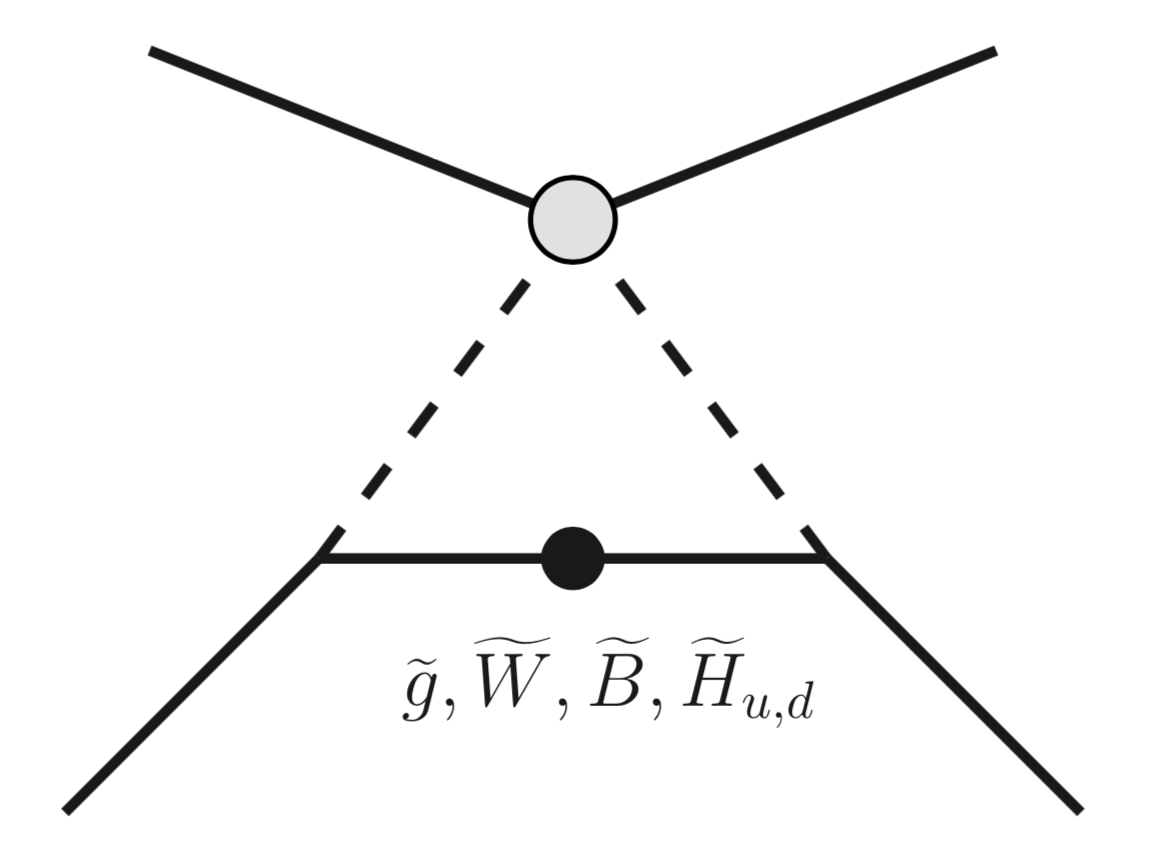
\includegraphics[width=6cm]{susy_matching.png}
\caption{1 loop diagram which contributes to matching SUSY dimension 5 operators to SMEFT dimension 6 operator. Grey dot is dimension 5 interaction, black dot is a gaugino/higgsino mass insertion. }
\label{fig:Fig1}
\end{center}
\end{figure}

\section{Flavor violation}

Before we give an explicit calculations for the different contributions, we must discuss flavor mixing in the MSSM. Soft SUSY breaking terms in general lead to large mixing between different sfermion generations. After diagonalizing the quark masses, and rotating to the Super-CKM basis the sfermion mass matrices have the following form:

\[
m_{\tilde{f}}^2 = m_{0}^{2}
  \begin{pmatrix}
    1 + \Delta_{1}^{\tilde{f}} & \delta_{12}^{\tilde{f}} & \delta_{13}^{\tilde{f}}\\
     \delta_{12}^{\tilde{f}*} & 1 + \Delta_{2}^{\tilde{f}} & \delta_{23}^{\tilde{f}}\\
      \delta_{13}^{\tilde{f}*} & \delta_{23}^{\tilde{f}*} & 1 + \Delta_{3}^{\tilde{f}}
  \end{pmatrix}
\]

where in $m_{\tilde{f}}^2$, $\tilde{f}$ stands for any sfermion. We can anticipate that each of the off diagonal terms will be small, and treat them as a perturbation using the mass insertion method. A priori, these off diagonal terms introduce large flavor-changing neutral currents (FCNC) and CP violation, severely constraining their values depending on the scale of supersymmetry breaking. 


One simplifying assumption to make is that of Minimal Flavor Violation (MFV). In this scenario, the only source of FCNC and CP violation in the MSSM is from the CKM matrix. In MFV, we can diagonalize the fermion and sfermion mass matrices via the same field redefinitions, and the off diagonal terms of $m_{\tilde{f}}^2$ are zero. For what follows we assume MFV, but will comment on the affect of flavor mixing.

\section{Loop Contributions}

First we will define the loop function $F(m_{1},m_{2},M)$

\begin{align}
F(m_{1},m_{2},M) = &\int \frac{\text{d}^{4}l}{(2\pi)^{4}} \frac{M}{(l^2 - m_{1}^{2})(l^2 - m_{2}^{2})(l^2 - M^{2})}\nonumber \\
&\frac{iM}{16}\left(\frac{m_{1}^{2}M^{2}ln(\frac{m_{1}^{2}}{M^{2}}) + m_{1}^{2}m_{2}^{2}ln(\frac{m_{2}^{2}}{m_{1}^{2}}) + m_{2}^{2}M^{2}ln(\frac{M^{2}}{m_{2}^{2}})}{(m_{1}^{2} - m_{2}^{2})(m_{1}^{2} - M^{2})(m_{2}^{2} - M^{2})}\right)
\end{align}

where M is the mass of the exchanged higgsino/gaugino. This loop function will appear in each of our contributions.

\subsection{Higgsino contributions to $P\rightarrow K^{+}\bar{\nu}$}
Diagrams like those in figure \ref{Fig1} where a Higgsino is exchanged are usually dominant. These give the matching conditions

\begin{enumerate}
\item $C_{RL}(uds\nu_{i}) = \sum_{j=1}^{3} \frac{g_{2}^{2}m_{e_{i}}m_{u_{j}}V_{j2}}{M_{W}^{2}\text{sin}2\beta}F(m_{\tilde{e}_{i}}, m_{\tilde{u}_{j}}, \mu) C^{ijkl}_{5R}(M_{S})$
\item $C_{RL}(usd\nu_{i}) = \sum_{j=1}^{3} \frac{g_{2}^{2}m_{e_{i}}m_{u_{j}}V_{j1}}{M_{W}^{2}\text{sin}2\beta}F(m_{\tilde{e}_{i}}, m_{\tilde{u}_{j}}, \mu) C^{ijkl}_{5R}(M_{S})$
\end{enumerate}

In each of the above expressions we've summed over the squark flavor, j, in the sfermion loop, but the stop quark contribution should dominate because of the large mass of the third generation fermions. Additionally, the contribution from $\nu_{i} = \nu_{\tau}$ will dominate, as $m_{\tau} \gg m_{\mu},m_{e}$.



















\end{document}